
%% bare_jrnl_compsoc.tex
%% V1.3
%% 2007/01/11
%% by Michael Shell
%% 04/05/10
%% Edited by Suleyman Muhammad
%% See:
%% http://www.michaelshell.org/
%% for current contact information.
%%
%% This is a skeleton file demonstrating the use of IEEEtran.cls
%% (requires IEEEtran.cls version 1.7 or later) with an IEEE Computer
%% Society journal paper.
%%
%% Support sites:
%% http://www.michaelshell.org/tex/ieeetran/
%% http://www.ctan.org/tex-archive/macros/latex/contrib/IEEEtran/
%% and
%% http://www.ieee.org/
\documentclass[11pt,onecolumn,cspaper,compsoc]{IEEEtran}

% *** GRAPHICS RELATED PACKAGES ***

\usepackage{graphicx}
\graphicspath{{/home/suleyman/Desktop/Survey_Wireless_Security/LaTex/pics/}}

\DeclareGraphicsExtensions{.eps, .pdf, .png, .jpeg}

\renewcommand{\thesection}{\Roman{section}}
\renewcommand{\thesubsection}{\thesection.\roman{subsection}}

\begin{document}
\title{Survey on Wireless Security:\\ Security Issues and Solutions}

\author{Suleyman~Muhammad\\\and Graduate~Computer~Engineer\\\and Villanova~University~Class~2010\\\and Villanova~Graduates~Class~2011}

% The paper headers
\markboth{Wireless Security Survey, October~2010}%
{Muhammad \MakeLowercase{\textit{et al.}}: WIreless Security Survey}

\IEEEcompsoctitleabstractindextext{%
\begin{abstract}
The rapid growth in the use of wireless systems for basic tasks such as browsing and web surfing to more important financial and business 
tasks warrants the need for varied levels of security over the wireless medium. Data sent over a wireless network is essentially in the open 
for everyone to listen. Malicious users can attempt to steal the identity of authorized users already connected to the network or listen in 
on allocated channels to gain secure information and data. When tackling the issue of \textit{Wireless Security} the issue of power consumption becomes 
significant. Since wireless users are often very mobile, their devices (hand helds, mobile phones, laptops) run on reserve power. With 
reserve power or battery power, the device in turn has limited transmission power and limited computing capabilities. And more so with the 
smaller devices there are hardware limitations which also hinder its processing power. These factors often make using weak, low power 
consuming cryptographic mechanisms the only sensible option. But one must decide whether to implement cryptographic security schemes in software 
at the risk of consuming excess ammounts of reserve power, or add special purpose hardware units designed to make that job specialized and/or 
localized. This survey paper delves into implementations of these aforementioned ideas proposed by various authors who introduce some new 
\textit{Wireless Security} techniques. These techniques hope to prove that with new lightweight security specific hardware models, a secure 
wireless network is very possible. A theoretical method of combining the previously mentioned models to essentially create an air tight
 \textit{Wireless Security} solution is also presented. 
 
\end{abstract}

% Note that keywords are not normally used for peer review papers.
\begin{IEEEkeywords}
\centering
Wireless Security, Biometric Passport, Firewall Security, TRNG, Smart Card, Tokens.
\end{IEEEkeywords}}

% make the title area
\maketitle


\section{Introduction}

Most current cryptographic methods such as AES, IDEA, etc. require very high processing power. This often makes them infeasible for use in 
mobile systems without significantly lowering the devices battery life. This survey attempts to effectively bypass that issue by taking much
burden off the mobile device and involve specific hosts, and devices who's sole existance is to uphold the security requirements needed
to have a trusted and efficient Wireless Network. But before we explain possible solutions it is important to dissect the problem at hand. 
\textbf{Section II} does just that by describing some basic but hindering attacks that affect Wireless Systems specifically. Because of the Wireless 
medium, different issues must be addressed and steps must be taken to provide security for the parties involved. \textbf{Section III} introduces the 
use of our own individual biological stamp that each and every person was born with, our fingerprint, as a personal identification/encryption system. 
The next section, \textbf{Section IV} is a description of an involved method of internal network security involving the use of multiple different 
security mechanisms brought together to make a fairly secure Wireless System. The proposed method requires firewalls, Smart Cards and cryptographic 
tokens all in succession. Finally \textbf{Section V} is the conclusion which contains final statements and gives an example of how each of these 
ideas can be combined into one all encompassing Wireless Security System.

\section{Wireless Security Issues}

\indent To be truly confident that a connection is secure one must be sure that they have accounted for any possible attack. These attacks 
occur on many levels and come in many ways, shapes, and forms. To find a solution we must first analyze the problem. Security issues are present 
in almost every layer of the TCP/IP model. When taking in account wireless over TCP, issues on the Host-to-Network and Network layers need to be 
taken care of because these security issues cannot be solved by traditional methods.[1] The rest of this section defines a few security issues 
within those previously mentioned Wireless TCP/IP layers. The subsequent sections hope to provide the means to combat such attacks to increase 
\textit{Wireless Network Security}.

\subsection*{Host-to-Network}

Host-to-Network layer Attacks, mainly due to the wireless medium, can greatly decrease the successful transmission of data. A DoS attack, is when 
a malicious unauthorized user floods a network with requests for data or a connection making it difficult for an authorized user to gain 
access. Similarly Radio Frequency Jamming attacks occur when a malicious user targets devices on narrow frequency bands (e.g. 2.403-2.48GHZ in 
Bluetooth) and attempt to produce extensive Interference by flooding the wireless medium with noise.[1]

\subsection*{Network Layer}

Network layer attacks can occur with use of unauthorized equipment such as Access Points and Mobile Devices. An unauthorized user in this case 
will gain access to secure information and will be able to hide their malicious actions posing as the owner of the machine. The other manner 
in which a Network layer attack can commence is if a malicious entity provides false information to a Mobile Host such as false packet routes. 
The intermediary malicious entity, after receiving the packet to be routed, can drop the packets, route them to wrong locations, or even keep 
the data for itself all while returning false acknowledgements that the packets were delivered. 


\section{Biometrical Passport}

\begin{figure}[!t]
  \centering
  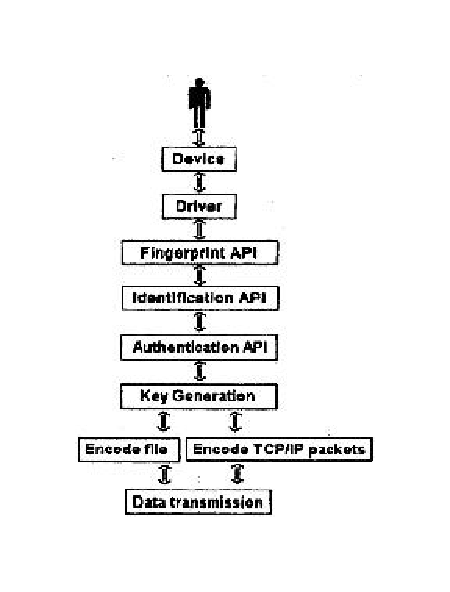
\includegraphics[scale=1]{BMpassprt}
  \caption{Biometrical Passport Model [2]}
  \label{BMP}
\end{figure}

The authors of [2] propose a new intuitive security model to deter malicious users who are intent on breaking into a wireless network. 
This model involves building software designed for encoding data transmitted through open radio channels using a biometrical passport. 
A biometrical passport, more commonly a fingerprint, is utilized to generate a specific 1.23 KB pattern read by a 
scanner. The scanner proposed is the Bio-Link U-Match scanner which will generate keys based on two inputs; first your fingerprint pattern, 
second a chosen keyword. Your data is encrypted with the generated key before being sent and this method assumes that public keys have been 
already been distributed between clients. The model shown in Figure \ref{BMP}. is that of the Biometrical Passport. The authors of [2] specify 
a few methods of data transfer in which this method would be practical, one being single file transmissions where services such as FTP (File 
Transfer Protocol), HTTP (HyperText Transfer Protocol), and SMTP (Single Message Transfer Protocol) will be used. For single file 
transmissions the Application layer uses the biometrical key to encode the data itself then transmits over the wireless medium. The second 
method is TCP/IP packet encryption which will require the help of the NDIS (Network Device Interface Specification) driver. With the NDIS 
driver transparent TCP/IP packet encryption and decryption between the Host-to-Network layer and the Network layer is possible.[2] Since some 
current systems already use fingerprints for access to the OS itself this could easily be implemented. It would definitely be a good use of 
resources to use the information provided as basic security to also provide the fingerprint for your wireless security.

\section{Wireless Internal Network Protection}

For Wireless Security, user privileges such as rlogin, telnet, and FTP can become a serious security issue. While crossing security 
domains one can possibly stumble onto an insecure channel. If this occurs while accessing the fore mentioned services hackers can possibly 
attain enough information to gain access to secure networks. Wireless security threats may be either internal or external. An 
\textit{Internal Network} is a group of mobile nodes or hosts all connected only at one point to the outside world a.k.a the \textit{External Network}.[3]

\begin{figure}[!ht]
  \centering
  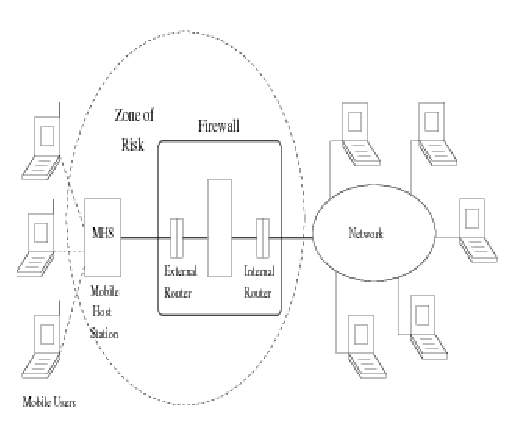
\includegraphics[scale=.9]{ZOR_w}
  \caption{Zone of Risk with Firewall [3]}
  \label{zorw}
\end{figure}

\begin{figure}[!ht]
  \centering
  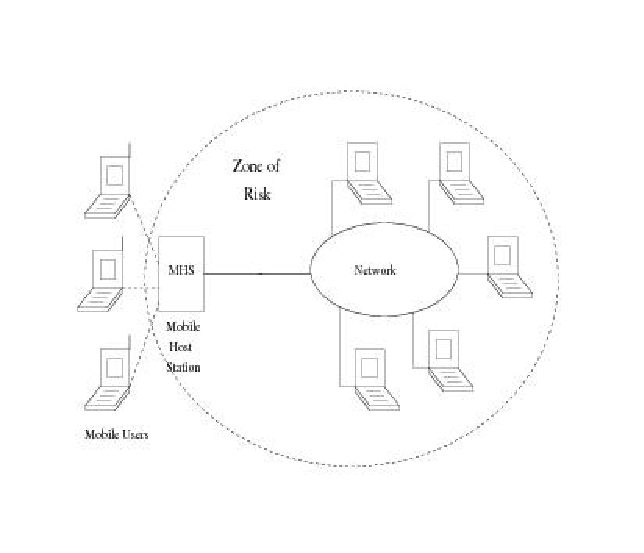
\includegraphics[scale=.9]{ZOR_wout}
  \caption{Zone of Risk without Firewall [3]}
  \label{zorwo}
\end{figure}

\subsection{3 Tiered Defence}

The authors of [3] propose a method which focuses on protection from external threats. They present the idea that security has two classes; 
That which is not expressly permitted is prohibited and that which is not expressly prohibited is permitted. The former and more secure 
of the two is known as a Pro-Active security mode and the latter is known as a Reactive security mode. For their security model the authors 
of [3] utilize a proactive mode wherein the System Administrator defines services that are used and searches each one of those services for 
security risks with high repetition. If the risk becomes too high, that service is restricted. A risk diagram is shown in Figure 
\ref{RE}. which could be used as a loose guide on how to handle risk since it can be difficult to quantify. The security model utilizes Firewalls to 
effectively design stern access controls. The goal of the model is to prevent intruders, but this method does not take in account unauthorized 
access from within the internal network. Though that may be true, what this method is successful in is protecting the network itself as well 
as the hosts who are connected and vulnerable to malicious attacks from the external world. Individual host protection is not required while 
within the network, again given there are no internal users who plan on causing trouble. This is due to the fact that the \textit{Zone of Risk} 
with and without a defensive firewall is very different as you can see in Figures \ref{zorw}. and \ref{zorwo}. respectively. Risk is 
significantly decreased and lies only within the firewall itself. Individual hosts are protected while connected to the internal network 
because the firewall forces all incoming traffic to be directed through one focal point. Any users who plan on causing mischief within the 
system will have a difficult time gaining access to the secure network.[3] 

\begin{figure}[!h]
  \centering
  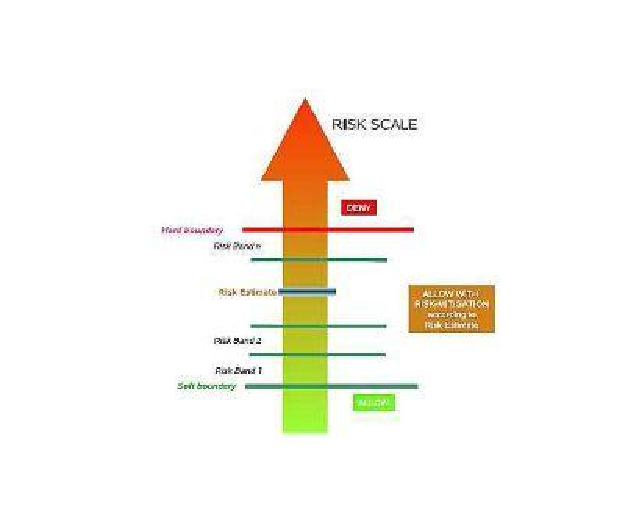
\includegraphics[scale=1]{Risk_Estimation}
  \caption{Risk Estimation Diagram [1]}
  \label{RE}
\end{figure}

\subsubsection*{Assumptions}

Firewalls are essentially a Hardware or Software barrier which is Inserted between an internal network and any external connections. External 
connections are often untrusted and possibly unwanted or harmful intrusions into the network in question. The implementation proposed by the 
authors of [3] have a few assumptions. First, encryption is assumed to be already implemented on data packets. Next there exists a mobile IP 
addressing scheme wherein a mobile device can move from network to network whilst keeping a permanent IP address. 
Any hosts attempting communication through nodes that are untrusted are denied access to the network. There are three main components to the 
proposed firewall, each providing its own level of defense so that if one component is conquered an attack must continue to the next level. 
At that next level corresponding component will be active to catch the intruder or at the very least temporarily halt their progress until 
the system administrator can identify that the network has been compromised. [3] 

\subsubsection*{TIER 1: External Screening Router}

The first component and also the first line of defense is the External Screening Router. The External Screening Router thoroughly examines 
incoming packets and determines which packets it will and will not allow. In this implementation packets are only allowed \textit(from) 
predetermined or approved Mobile IP addresses and \textit(to) intended addresses with an IP address of a trusted address 
(part of the network). Port numbers for incoming packets must be properly defined e.g. Telnet 23, HTTP 80. Obvious intruders are denied such 
as incoming packets that have a source address which is that of an internal network node. [3]

\subsubsection*{TIER 2: Administrative Host}

The second line of defense is the Bastion Host or Administrative Host which is essentially the heart of the firewall. The Administrative host 
is the focal point of all incoming and outgoing traffic and if a packet passes the screening router it must still pass the security checks of 
the Administrative Host. If Administrative host cannot handle the traffic load through the system, multiple firewalls should be implemented to 
allocate the task in a distributed fashion. Internal and External network users are not given any access to this host, essentially only the 
System Administrator and those of the like. Within the Administrative Host All programs not involved in the firewall functionality are removed 
and services which are not required are eliminated. The Administrative Host is capable of application level support such as email forwarding 
and DNS queries. Requests from privileged services such as FTP, telnet, and rlogin are processed and either allowed or denied with prejudice. 
The Administrative Host has a registry of security issues and security rules are dynamic. This means that they can adapt to varied security 
events.[3]

\subsubsection*{TIER 3: Internal Screeing Router}

The last line of defense before the entire network is exposed and in turn compromised, is the \textit{Internal Screening Router}. The basic strengths and weaknesses of the 
\textit{Internal Screening Router} are equal to that of the \textit{External Screening Router}. It provides internal protection from from the \textit{External Screening Router} as well as from 
the \textit{Administrative Host}, in case the security of the \textit{Administrative Host} becomes compromised. All packets are screened before being sent throughout the internal network.[3]

\subsection{Smart Card, Challenge-Response, and Crytographic Tokens}

Most implementations of current security protocols store sensitive data concerning the said protocol within the OS itself but this lowers the portability because this information must be 
transferred from host to host. Also issues arise when sensitive data is stored in public areas because worms, Trojans and malicious applications of the like have the capabilities of accessing 
this data while the OS is performing its duties.[5] The authors of [3] and [5] propose that \textit{Smart Cards} are the solution for this. \textit{Smart Cards} are perfect for storing cryptographic keys and 
algorithms and can be implemented without having to change the current security standard used by the 802.11i Task Group.[5] Shortcomings of the firewall approach leave holes in internal network 
protection or more specifically protection from alleged internal users. Node Addresses are all static and an intuitive intruder could effectively intercept and pose as an internal node using 
that IP addressing. Also mobile devices can be stolen and used directly as an authorized node and something needs to be done about these internal security issues. This is where the 
\textit{Smart Card} can be used most efficiently.[3]

\subsubsection*{Smart Card}

Smart Cards are small credit card sized computing device inserted into mobile computers within the internal network. This is not only a form of security, but also serves to keeps the amount of 
users on the network to a controlled value. Each Smart Card can be replaced by the System Administrator whenever they feel the system has a security breach. Each Smart Card has an independent 
processor which can perform special cryptographic calculations. The Smart Cards are integral devices for machine verification if used in accordance with the authors’ proposed Challenge-Response 
verification method.[3]

\subsubsection*{Challenge-Response}
In Challenge-Response the Administrative Host sends a random number or as the authors of [3] call it a “challenge” to the mobile device in question. The mobile device being challenged must 
reply with the corresponding “response” or the connection will be ended. Smart card calculates the response unnoticed by the user using one or multiple protected algorithms, possibly similar to 
AES or RSA methods of message encryption/decryption. Challenge-Response is performed during initial connection to internal network and when a mobile computer is attempting operations deemed 
protected by the system administrator. Also for added security, Challenge-Response is performed at random times to quickly catch rouge users trying to assume the identity of an internal node.[3]

\subsubsection*{Cryptographic Token Device}

Since reusable passwords are sent over a wireless medium they are essentially insecure. An added precaution to combat this comes with the Token. The Token is a small hand-held cryptographic 
device each user must carry to access the system which performs an unknown calculation similar to the smart card. The authors of [3] propose that a challenge-response is used also on the user 
level using the Token. But the user level challenge-response must utilize different algorithms than that of machine verification. When an attempt to access the wireless network is approved the 
Administrative Host then sends a challenge key to that mobile computer. The user must input that key into their personal Token and the Token will return the corresponding response to the 
challenge which must be inputted to the mobile device by the user. This will be done for initial connections as well when requests to perform “protected operations” are initiated. [3]

\begin{figure}[!h]
  \centering
  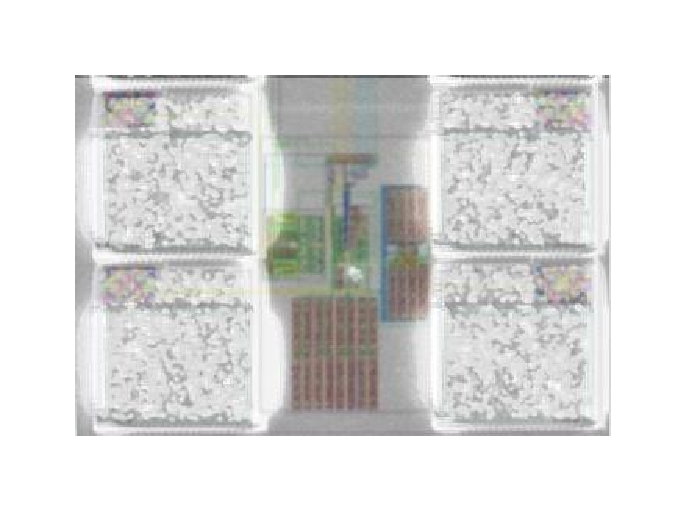
\includegraphics[scale=.8]{TRNGchip}
  \caption{TRNG Chip Micro Image}
  \label{chip}
\end{figure}

\subsubsection*{True Random Number Generation}

Random number generation is often the make or break factor in cryptography. Since traditional Random Number Generators use algorithms to create random numbers, they are not actually random at 
all but pseudo random since they can be easily recreated with the same initial conditions. A hacker who wants to break into your system or wants to take a look at your encrypted messages needs 
only to know the initial conditions used for random generation and the algorithm used for encryption. To enhance any security system, not only wireless networks, the introduction of true 
randomness can make all the difference. This makes any intruders attempts on the system almost impossible because the same conditions cannot be recreated. True random number generation (TRNG) 
as the authors of [6] have determined can be created using samples of device noise. This increases security level significantly. If this method is used in each step of random generation 
for the proposed Firewall method this will make an already strong system, impenetrable. The authors of [6] have formulated a low power CMOS implementation of this random number generator. The 
circuit is fabricated in a 0.12 nano meter digital CMOS technology with an area of 9000 nano square meters Figure \ref{chip}. The total power consumption is 50 nano WATTS for 200 kb/s true 
random output data. The power distribution is 20 nano Watts of DC-power and 30 nano Watts/MHz for clocked power which depends on sampling frequency. With low power consumption and a small layout 
area this method is very feasible in small devices such as the proposed Tokens and Smart Cards to create a fully protected netowrk.

\section{Conclusion}

Wireless Security is far from impossible. The only difference is that security of a Wireless System depends on physical security issues as well as thoes involved with traditional 
wire-line networks. The firewall method proposed by the authors of [3] can definately be implemented on any system whether it is wireless or wired. With the inevitable switch to IPv6, mobile IP
addressing is a strong possibility, making this method even more attractive. The firewall, as long as it is intact and uncompromised, can very effectively guarantee the saftey of the internal 
network from external attacks. At that point the internal network can focus its resources on internal security by requiring machine verification using the Smart Card, and user verification using 
the crytographic token. The Smart Card and Cryptographic Tokens can both be solidified as secure verification tools once they have implemented True Random Generation with the help of the proposed 
microchip which uses device noise as its source. To complete the system we add the security of a strictly personal biometrical key for encryption of any data transfers. Lastly, 
for the proposed system's implementation we can use a fingerprint as an input to the Cryptographic Token which can also be an effective use of resources. The final issue that must be 
addressed is that this implementation is in fact theoretical and its actual implementation may be very costly financially as well as taxing on the system itself. But with that being said, for 
systems that need maximum levels of security, and would benifit from the usage of wireless networks will definitely find that this method, if properly designed and created would be worth the expense.  
  


\section*{Acknowledgment}

I would like to thank Professor Sarvesh for his guidance. I would also like to thank Debra Galloway, Keshia Pershad, and my family for their unequivocated support. Without them this would not be possible.




\newpage
\begin{thebibliography}{1}


\bibitem{WIL}
M. Srivatsa, "Who is Listening? Security in Wireless Networks," \emph{IEEE International Conference on Signal Processing, Communications and Networking, 2008. ICSCN '08}, pp. 167-172, 07 Feb. 2008, doi:10.1109/ICSCN.2008.4447182.

\bibitem{BioPass}
D.V. Vishnyakov, A.G. Serdyukov, "Cryptographic data security in wireless networks based on biometrical passport," \emph{IEEE International Siberian Conference on Control and Communications, 2005. SIBCON '05.}, pp. 52-54, 03 Apr. 2006, doi:10.1109/SIBCON.2005.1611191.

\bibitem{FREwall}
U. Murthy, O. Bukhres, W. Winn, and E. Vanderdez. "Firewalls for security in wireless networks," \emph{Proc. 31st Hawaii International Conference on System Sciences, 1998. HICSS '08}, vol. 7, pp. 672-680, 06 Aug. 2002, doi:10.1109/HICSS.1988.649269.

\bibitem{Pconsumption}
D. Meintanis, I. Papaefstathiou, "On the Power Consumption of Security Algorithms Employed in Wireless Networks," \emph{6th IEEE  Consumer Communications and Networking Conference, 2009. CCNC '09.}, pp. 1-5, 18 Feb. 2009, doi:10.1109/CCNC.2009.4784732.

\bibitem{EnhSec}
S. Koutroubinas, T. Karoubalis, P. Rozos, and P. Nastou, "Enhancing security in wireless networks," \emph{IEEE International Symposium on Consumer Electronics, 2004.}, pp. 214-218, 10 Jan. 2005, doi:10.1109/ISCE.2004.1375939.

\bibitem{TRNGb}
R. Brederlow, R. Prakash, C. Paulus, and R. Thewes, "A low-power true random number generator using random telegraph noise of single oxide-traps," \emph{IEEE International Solid-State Circuits Conference, 2006. ISSCC '06}, pp. 1666-1675, 18 Sept. 2006, doi:10.1109/ISSCC.2006.1696222.

%%\bibitem{mobie_nav_bot}
%%M.A. Batalin, G.S. Sukhatme, and M. Hattig, "Mobile Robot Navigation Using a Sensor Network," \emph{Proc. IEEE International Conference on Robotics and Automation, 2004.}, vol.1, pp. 636-641, Apr. 2004, doi:10.1109/ROBOT.2004.1307220.

\end{thebibliography}

\end{document}
